\documentclass{article}
\usepackage[utf8]{inputenc}
\usepackage[acronym,nomain,nonumberlist]{glossaries}
\usepackage{enumitem}
\usepackage{amsfonts}
\usepackage{amssymb}
\usepackage{hyperref}
\usepackage{wrapfig}
\usepackage{graphicx}
\graphicspath{ {images/} }

\makeglossaries

\newacronym{AI}{AI}{Artificial Intelligence}
\newacronym{BI-RADS}{BI-RADS}{Breast Imaging Reporting and Data System}
\newacronym{CC}{CC}{CranioCaudal}
\newacronym{CFA}{CFA}{Confirmatory Factor Analysis}
\newacronym{DICOM}{DICOM}{Digital Imaging and Communications in Medicine}
\newacronym{DOTS}{DOTS}{Dimensions Of Trust Scale}
\newacronym{HAII}{HAII}{Human-AI Interaction}
\newacronym{MG}{MG}{MammoGraphy}
\newacronym{MLE}{MLE}{MaximumLikelihood Estimation}
\newacronym{MLO}{MLO}{MedioLateral Oblique}
\newacronym{MM}{MM}{Multi-Modality}
\newacronym{MRI}{MRI}{Magnetic Resonance Imaging}
\newacronym{NASA-TLX}{NASA-TLX}{NASA Task Load Index}
\newacronym{SEM}{SEM}{Structural Equation Modeling}
\newacronym{SS}{SS}{Single-Modality}
\newacronym{SUS}{SUS}{System Usability Scale}
\newacronym{UI}{UI}{User Interface}
\newacronym{US}{US}{UltraSound}
\newacronym{UTA}{UTA}{User Testing and Analysis}
\newacronym{UTAUT}{UTAUT}{Unified Theory of Acceptance and Use of Technology}

\hypersetup{
    colorlinks=true,
    linkcolor=black,
    filecolor=black,
    urlcolor=black,
    citecolor=black,
}

\title{
MIDA
\\
User Testing \& Analysis Guide
\\
Clinical Opinion About Intelligent Agents
\\
}

\author{
Francisco Maria Calisto\\
\texttt{francisco.calisto@tecnico.ulisboa.pt}\\
Instituto Superior T\'{e}cnico\\
University of Lisbon\\
Portugal
}

\date{21/11/2019}

\begin{document}

\maketitle

\textbf{BreastScreening:} \hfill \href{https://breastscreening.github.io/}{breastscreening.github.io}

\textbf{Meta:} \hfill \href{https://github.com/BreastScreening/meta}{github.com/BreastScreening/meta}

\textbf{Datasets:} \hfill \href{https://github.com/BreastScreening/meta/wiki/Datasets}{github.com/BreastScreening/meta/wiki/Datasets}

\hfill

\textbf{MIDA:} \hfill \href{https://mida-project.github.io/}{mida-project.github.io}

\textbf{Meta:} \hfill \href{https://github.com/mida-project/meta}{github.com/mida-project/meta}

\textbf{Datasets:} \hfill \href{https://github.com/mida-project/meta/wiki/Datasets}{github.com/mida-project/meta/wiki/Datasets}

\hfill

\textbf{MIMBCD-UI:} \hfill \href{https://mimbcd-ui.github.io/}{mimbcd-ui.github.io}

\textbf{Meta:} \hfill \href{https://github.com/MIMBCD-UI/meta}{github.com/MIMBCD-UI/meta}

\textbf{Datasets:} \hfill \href{https://github.com/MIMBCD-UI/meta/wiki/Datasets}{github.com/MIMBCD-UI/meta/wiki/Datasets}

\clearpage

%%%%%%%%%%%%%%%%%%%%%%%%%%%%%%%%%%%%%%%%%%%%%%%%%%%
%                                                 %
%                     SECTION                     %
%                                                 %
%%%%%%%%%%%%%%%%%%%%%%%%%%%%%%%%%%%%%%%%%%%%%%%%%%%

\section{Introduction}
\label{sec:sec001}

%%%%%%%%%%%%%%%%%%%%%%%%%%%%%%%%%%%%%%%%%%%%%%%%%%%

During the breast cancer screening, missing cancers may not be identified until they are more advanced and less agreeable to treatment~\cite{Houssami2017}.
Artificial Intelligence (AI) in the medical workflows may help with this challenge~\cite{McKinney2020}.
Studies have demonstrated the ability of AI to meet the human's performance on various clinical tasks~\cite{info:doi/10.2196/10010, Topol2019}.
As a lack of medical professionals threatens the adequacy and availability of clinical services worldwide~\cite{doi:10.1002/j.2051-3909.2012.tb00169.x, rimmer2017radiologist}, the scalability of AI could improve to higher care.

The role of Human-AI Interaction (HAII) in healthcare delivery the appropriate settings in which it can be applied, and its impact on the quality of care have yet to be evaluated~\cite{Tschandl2020}.
There have been several attempts at addressing the effects of HAII across multiple workflows and different levels of clinical expertise~\cite{doi:10.1148/radiol.2019182627, doi:10.1148/ryai.2020200057}.
However, the use case of breast cancer diagnosis to address the effects from varied representations of AI-based supported by intelligent agents is still scarce.
This explains why it is an open topic research, and the motivation behind the proposed research of this User Testing and Analysis (UTA) guide.
%%%%%%%%%%%%%%%%%%%%%%%%%%%%%%%%%%%%%%%%%%%%%%%%%%%
%                                                 %
%                     SECTION                     %
%                                                 %
%%%%%%%%%%%%%%%%%%%%%%%%%%%%%%%%%%%%%%%%%%%%%%%%%%%

\section{Description}
\label{sec:sec002}

This document describes our test plan for conducting our user tests during the development of the \hyperlink{https://breastscreening.github.io/}{BreastScreening} project and systems. The goals of the user testing phases include establishing a baseline of participant performance, establishing and validating participant performance measures, and identifying potential design concerns to be addressed in order to improve the efficiency, productivity, and end-user satisfaction within the development and introduction of \textit{AI-Assistive} methods inside the Radiology Room (RR), between others, for Medical Imaging (MI), or more precisely, the breast cancer diagnosis.

%%%%%%%%%%%%%%%%%%%%%%%%%%%%%%%%%%%%%%%%%%%%%%%%%%%

\hfill

The user test objectives are:

\begin{enumerate}
\item To determine design inconsistencies and issues within the UI and content areas;
\begin{enumerate}
\item \textbf{Navigation Errors};
\item \textbf{Presentation Errors};
\item \textbf{Control Usage Problems};
\end{enumerate}
\item Exercise the prototype under controlled test conditions with representative users;
\item Establish baseline user performance and user-satisfaction levels of the user interface for future usability evaluations;
\end{enumerate}

%%%%%%%%%%%%%%%%%%%%%%%%%%%%%%%%%%%%%%%%%%%%%%%%%%%

Potential sources of error may include: (a) \textbf{Navigation Errors:} failure to locate functions, excessive keystrokes to complete a function, failure to follow recommended screen flow; (b) \textbf{Presentation Errors:} failure to locate and properly act upon desired information in screens, selection errors due to labeling ambiguities; and (c) \textbf{Control Usage Problems:} improper toolbar or entry field usage. Data will be used to access whether usability goals regarding an effective, efficient, and well-received user interface have been achieved.

To verify our work, we identified measurable and explicit targets. By having several goals, including that a value percentage of the users should be able to operate the tasks without the need of help. On the same rate value, the user should be able to start and complete the medical diagnosis tasks over the system with little errors or mitigating those errors. Measuring the expected number of errors with a relation between pilot \hyperlink{https://github.com/MIMBCD-UI/testing-guide-breast/tree/master/samples/test_4}{early} tests. On the laboratory pilot tests we aim to test our prototypes with researchers.

Researchers are in the context of the system, and know well the functionalities, so that, we need to expect a percentage value over their results compared to clinicians and not the same benefits. Last but not least, both users (researchers and clinicians) should be able to understand in a similar time amount the meaning of all visible controls. By the similar amount of time, it is expected to have a variance of the percentage value between researchers and clinicians, as well as values of early tests, of the same value percentage of the early goals described in this paragraph.

We tested each objective in early laboratory and field tests, so that we could take the appropriate corrective actions. Also, we expect to run early field tests with researchers and clinicians to highlight issues that we overlooked and ignored during the prototyping phase. To support interaction use by the participants, we will try to emphasize several key factors on our user tests. The tasks must be simple, low intrusive, support for natural interaction and the system must always give visibility and the task current-state.
%%%%%%%%%%%%%%%%%%%%%%%%%%%%%%%%%%%%%%%%%%%%%%%%%%%
%                                                 %
%                     SECTION                     %
%                                                 %
%%%%%%%%%%%%%%%%%%%%%%%%%%%%%%%%%%%%%%%%%%%%%%%%%%%

\section{Methodology}
\label{sec:sec003}

%%%%%%%%%%%%%%%%%%%%%%%%%%%%%%%%%%%%%%%%%%%%%%%%%%%
%%%%%%%%%%%%%%%%%%%%%%%%%%%%%%%%%%%%%%%%%%%%%%%%%%%
%                                                 %
%                     SECTION                     %
%                                                 %
%%%%%%%%%%%%%%%%%%%%%%%%%%%%%%%%%%%%%%%%%%%%%%%%%%%

\section{Roles}
\label{sec:sec004}

The roles involved in our user tests are as follows. An individual may play multiple roles, as well as the test may not require all roles.

\subsection{Trainer}

\begin{itemize}
\item Provide training overview prior to user testing phases;
\end{itemize}

\subsection{Facilitator}

\begin{itemize}
\item Provides overview of study to participants;
\item Defines tasks and purpose of the user testing to participants;
\item Assists in conduct of participant and observer debriefing sessions;
\item Responds to participant's requests for assistance;
\end{itemize}

\subsection{Data Logger}

\begin{itemize}
\item Records participant's actions and comments;
\end{itemize}

\subsection{Test Observers}

\begin{itemize}
\item Silent observer;
\item Assists the data logger in identifying problems, concerns, coding bugs and procedural errors;
\item Serve as note takers;
\end{itemize}

\subsection{Ethics}

All persons involved with the Usability (Usa.) test are required to adhere to the following ethical guidelines:

\begin{itemize}
\item The performance of any test participant must not be individually attributable;
\item Individual participant's name should not be used in reference outside the testing session;
\item A description of the participant's performance should not be reported to his or her superior;
\end{itemize}
%%%%%%%%%%%%%%%%%%%%%%%%%%%%%%%%%%%%%%%%%%%%%%%%%%%
%                                                 %
%                     SECTION                     %
%                                                 %
%%%%%%%%%%%%%%%%%%%%%%%%%%%%%%%%%%%%%%%%%%%%%%%%%%%

\section{Apparatus}
\label{sec:sec005}

%%%%%%%%%%%%%%%%%%%%%%%%%%%%%%%%%%%%%%%%%%%%%%%%%%%
%%%%%%%%%%%%%%%%%%%%%%%%%%%%%%%%%%%%%%%%%%%%%%%%%%%
%                                                 %
%                     SECTION                     %
%                                                 %
%%%%%%%%%%%%%%%%%%%%%%%%%%%%%%%%%%%%%%%%%%%%%%%%%%%

\section{Evaluation}
\label{sec:sec006}

The study followed the required ethical standards.
Specifically, the study complies with the provisions of the General Data Protection Regulation [Regulation (EU) 2016/279 of the European Parliament and of the Council of 27 April 2016], and follows the recommendations of the Declaration of Helsinki for research.
There are no risks and benefits associated with the users' participation.
User's participation is completely voluntary.

Quantitative and qualitative studies will be conducted with clinical experts and healthcare professionals.
Analysis will be performed by descriptive categorization statistics of statements.
In this document, results (Section~\ref{sec:sec011}) are being briefly described, but the evaluation process is further reported.

The raw data will be analyzed as follows.
In accordance with the recommendations of the two-stage procedure~\cite{rahi2018investigating}, CFA will be used to test validity and reliability of the model~\cite{crede2019questionable}.
SEM will be used as a preferable technique to regression as it allows simultaneous analysis of all relationships through multiple regression, while also allowing for both observed and latent variables to be analyzed at the same time, and providing overall fit statistics~\cite{hair2017advanced}.

%%%%%%%%%%%%%%%%%%%%%%%%%%%%%%%%%%%%%%%%%%%%%%%%%%%
%%%%%%%%%%%%%%%%%%%%%%%%%%%%%%%%%%%%%%%%%%%%%%%%%%%
%                                                 %
%                     SECTION                     %
%                                                 %
%%%%%%%%%%%%%%%%%%%%%%%%%%%%%%%%%%%%%%%%%%%%%%%%%%%

\section{Tasks}
\label{sec:sec007}

During our user tests, we need to ask participants to provide a subjective assessment of their experience using our \textit{Assistant}. There are several widely used questionnaires giving us different prons-and-cons. However, in most cases, a \hyperlink{https://www.nngroup.com/articles/keep-online-surveys-short/}{single question instrument}~\cite{sauro201210} is the right method for a quantitative usability testing. By taking less time and effort to answer, participants are pursuing to this phase after task, while it is minimally disruptive.

\clearpage

The tasks were derived from test scenarios ({\it i.e.}, {\bf Sce1.} and {\bf Sce2.}) developed from use cases and/or with the assistance of a subject-matter expert.  Due to the range and extent of functionality provided in the system, and the short time for which each participant will be available, the tasks are the most common and relatively complex for the available functions. The tasks are identical for all participants of a given user role in the study.

At this stage, each participant will interact with our UI. The UI show to each participant the set of patients chosen randomly (Section \ref{sec:sec001}). The set of patients will provide participants with 50 patients, while all patients much have at least one of the three available modalities (Figure \ref{fig:svmm}). Each participant will open each patient ({\it e.g.}, {\bf Pat1.}, {\bf Pat2.} or {\bf Pat3.}), of the three patients chosen randomly, and will examine the set of images. During examination, the participant will interact with the available features (Section \ref{sec:sec005}) of the system.

%%%%%%%%%%%%%%%%%%%%%%%%%%%%%%%%%%%%%%%%%%%%%%%%%%%

\hfill

\begin{wrapfigure}{r}{0.50\textwidth}
\centering
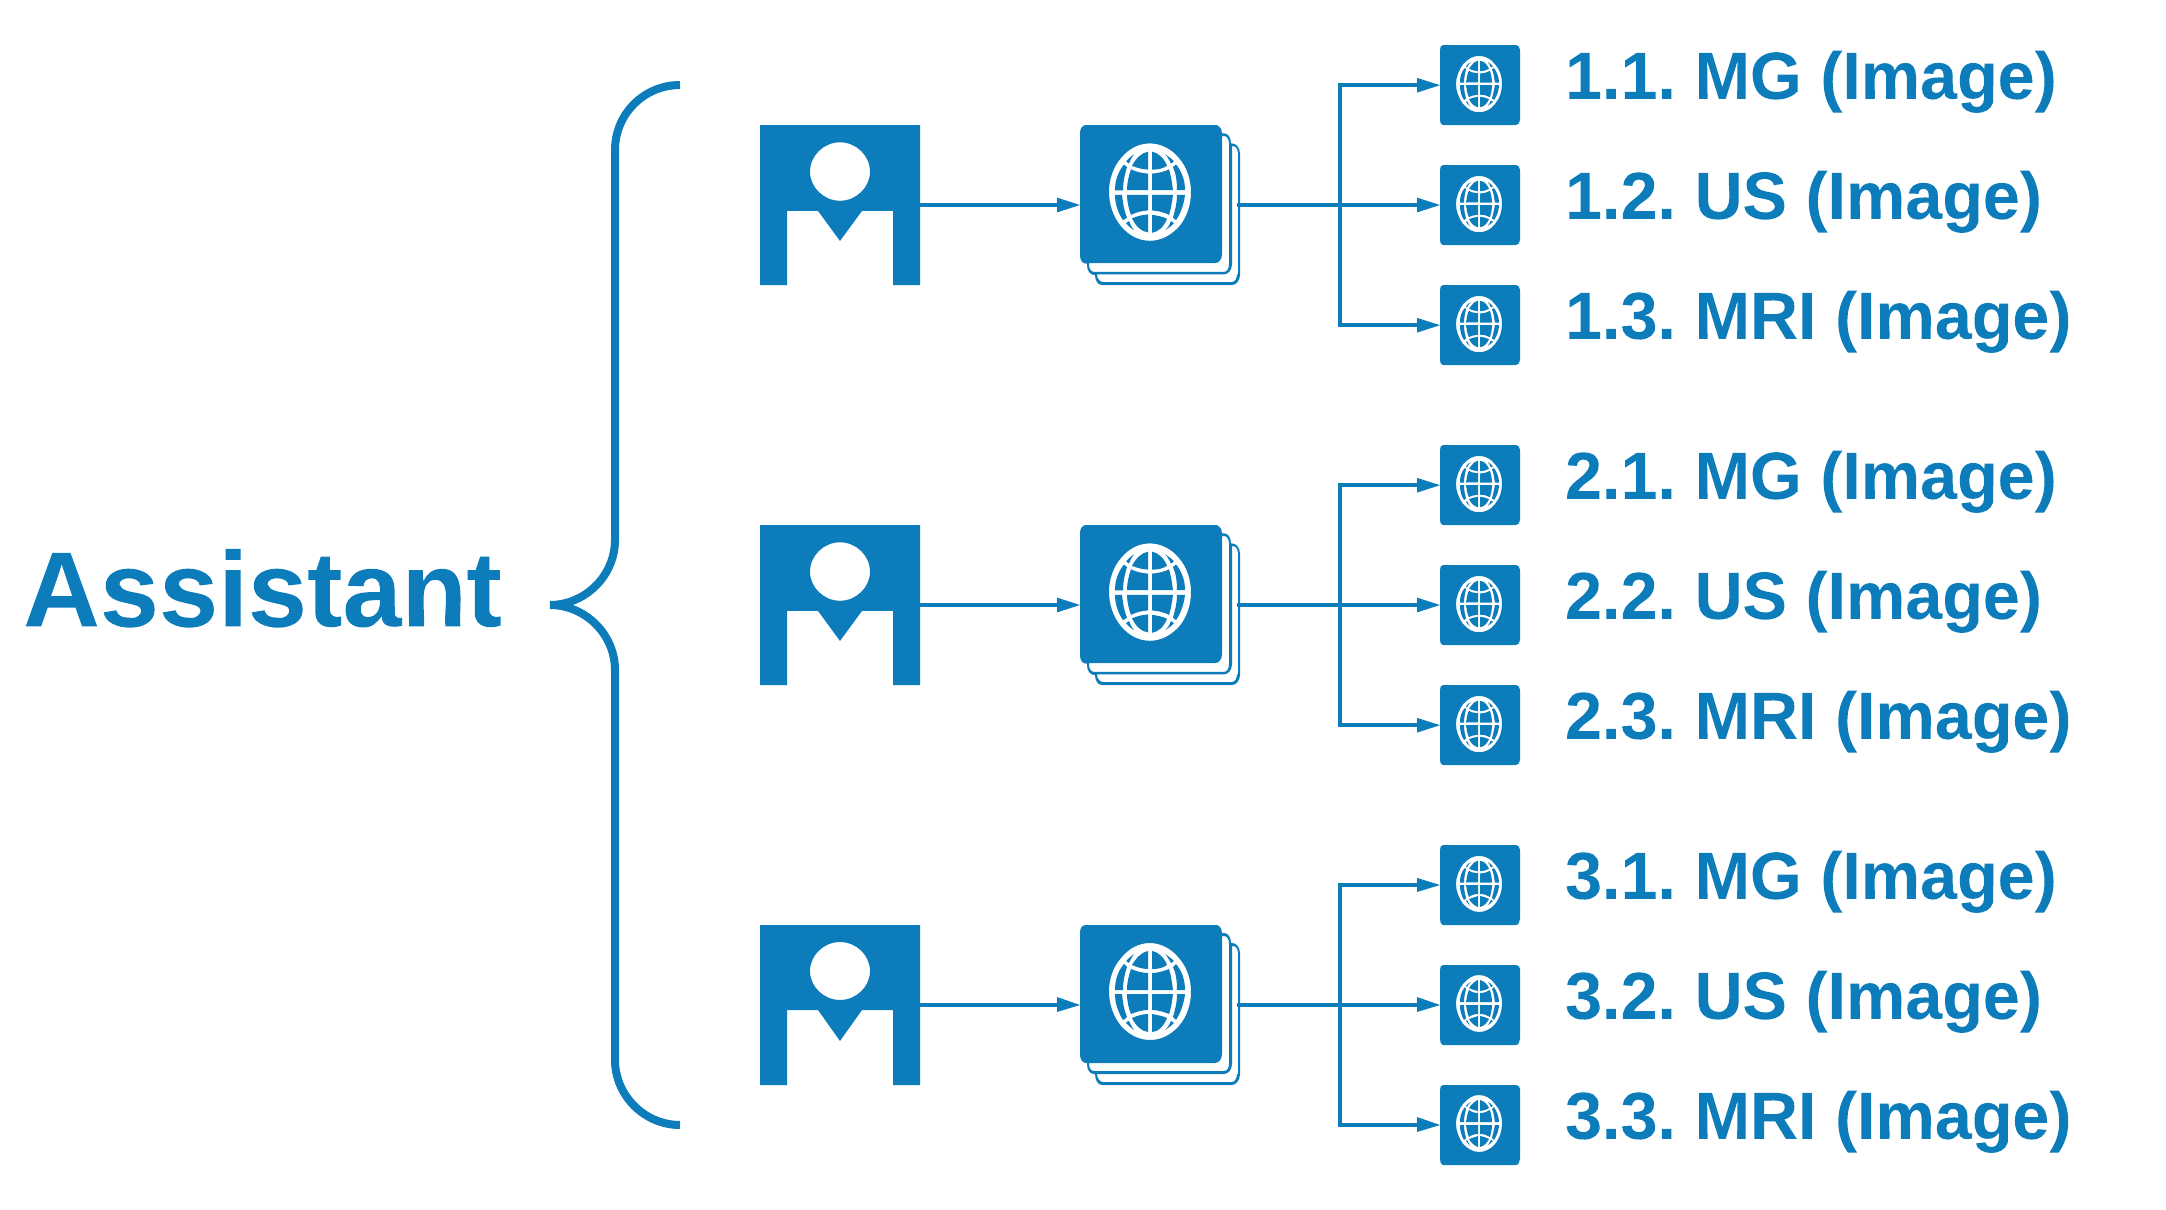
\includegraphics[width=0.50\textwidth]{img001}
\caption{Diagram representing the use of the \textit{Assistant} by clinicians. Each patient can have, and is not limited to have more images per modality.}
\label{fig:svmm}
\end{wrapfigure}

\hfill

%%%%%%%%%%%%%%%%%%%%%%%%%%%%%%%%%%%%%%%%%%%%%%%%%%%

We will try to understand if, with the \textit{AI-Assisted} techniques, the clinicians will encounters the most accurate severity (\hyperlink{https://en.wikipedia.org/wiki/BI-RADS}{BIRADS}) of the breast lesions~\cite{american1998breast} and patient's prognostic. For this purpose, we have several patients (Figure \ref{fig:svmm}); each patient has several images in the respective modalities: (i) \gls{MG}; (ii) \gls{US}; and (iii) \gls{MRI}. The clinicians will proceed to the activity of diagnosing three random patients within the support of our \textit{Assistant} by the observation of all images.

\hfill

In our \textit{User Testing Guide} a set of tasks is necessary and carefully crafted. Our test studies involve asking participants to perform a set of tasks. By looking at what our user need to do with our system, our tasks are realistic as possible. We are not describing the exact steps participants need to take. We achieve that by avoiding the precise language used as labels in our system. The tasks are emotionally neutrals. And we did several \hyperlink{https://www.nngroup.com/articles/pilot-testing/}{pilot tests} to prevent misleading situations saving us from wasting resources by accidentally use a lousy task or from getting bad data. The tasks are as follows.

The task descriptions below are required to be reviewed by all researchers and facilitators (Section \ref{sec:sec004}) to ensure that the content, format, and presentation are representative of real use and substantially evaluate the total system. Their acceptance is to be documented prior to the user test. Each task, is related to the set of {\it Phases}, {\it Scenarios} and {\it Activities} (Section \ref{sec:sec001}) on the next section (Section \ref{sec:sec008}) further explained.

\clearpage

%%%%%%%%%%%%%%%%%%%%%%%%%%%%%%%%%%%%%%%%%%%%%%%%%%%

List of stand alone tasks for both {\bf Pha1.}, {\bf Pha2.} and {\bf Pha3.} phases:

%%%%%%%%%%%%%%%%%%%%%%%%%%%%%%%%%%%%%%%%%%%%%%%%%%%

\hfill

\begin{itemize}
\item[] \textbf{Task 1.1.1:} Fill the Consent Form (Section \ref{sec:sec001}) and accept the user test;
\item[] \textbf{Task 1.1.2:} Fill the User Characterization Form (Section \ref{sec:sec001}) and proceed;
\end{itemize}

\hfill

\begin{itemize}
\item[] \textbf{Task 2.1.1:} Classify \textit{Patient 1} ({\bf Pat1.}) on the {\it \gls{MM}} condition;
\item[] \textbf{Task 2.1.2:} Classify \textit{Patient 2} ({\bf Pat2.}) on the {\it \gls{MM}} condition;
\item[] \textbf{Task 2.1.3:} Classify \textit{Patient 3} ({\bf Pat3.}) on the {\it \gls{MM}} condition;
\end{itemize}

\hfill

\begin{itemize}
\item[] \textbf{Task 2.2.1:} Freely explore \textit{Patient 1} ({\bf Pat1.}) on the {\it \gls{MM}} condition;
\item[] \textbf{Task 2.2.2:} Freely explore \textit{Patient 2} ({\bf Pat2.}) on the {\it \gls{MM}} condition;
\item[] \textbf{Task 2.2.3:} Freely explore \textit{Patient 3} ({\bf Pat3.}) on the {\it \gls{MM}} condition;
\end{itemize}

\hfill

\begin{itemize}
\item[] \textbf{Task 2.3.1:} Work. \& Usa. questions for the {\it \gls{MM}} condition;
\item[] \textbf{Task 2.3.2:} {\it Post-task} questions for the {\it \gls{MM}} condition;
\end{itemize}

\hfill

\begin{itemize}
\item[] \textbf{Task 3.1.1:} Classify \textit{Patient 1} ({\bf Pat1.}) on the \textit{Assis.} condition;
\item[] \textbf{Task 3.1.2:} Classify \textit{Patient 2} ({\bf Pat2.}) on the \textit{Assis.} condition;
\item[] \textbf{Task 3.1.3:} Classify \textit{Patient 3} ({\bf Pat3.}) on the \textit{Assis.} condition;
\end{itemize}

\hfill

\begin{itemize}
\item[] \textbf{Task 3.2.1:} Freely explore \textit{Patient 1} ({\bf Pat1.}) on the \textit{Assis.} condition;
\item[] \textbf{Task 3.2.2:} Freely explore \textit{Patient 2} ({\bf Pat2.}) on the \textit{Assis.} condition;
\item[] \textbf{Task 3.2.3:} Freely explore \textit{Patient 3} ({\bf Pat3.}) on the \textit{Assis.} condition;
\end{itemize}

\hfill

\begin{itemize}
\item[] \textbf{Task 3.3.1:} Work., Usa. \& Trust questions for the \textit{Assis.} condition;
\item[] \textbf{Task 3.3.2:} {\it Post-task} questions for the \textit{Assis.} condition;
\end{itemize}

\hfill

%%%%%%%%%%%%%%%%%%%%%%%%%%%%%%%%%%%%%%%%%%%%%%%%%%%
%%%%%%%%%%%%%%%%%%%%%%%%%%%%%%%%%%%%%%%%%%%%%%%%%%%
%                                                 %
%                     SECTION                     %
%                                                 %
%%%%%%%%%%%%%%%%%%%%%%%%%%%%%%%%%%%%%%%%%%%%%%%%%%%

\section{Metrics}
\label{sec:sec008}

Our user test metrics refers to user performance measured against specific performance goals necessary to satisfy the test requirements. Scenario completion success rates, adherence to dialog scripts, error rates, and subjective evaluations will be used. Time-to-Completion (TtC)~\cite{ioannidis1998effect} of scenarios will also be collected. From the set of tasks (Section \ref{sec:sec007}), each task corresponds to the set of {\it Phases}, {\it Scenarios} and {\it Activities} (Section \ref{sec:sec001}), meaning that we first need to explain it relations.

The first two tasks, {\it i.e.}, {\bf Task 1.1.1} and {\bf Task 1.1.2}, are related to the {\bf Pha1.} phase, as well as with {\bf Act1.}, {\bf Act2.} and {\bf Act3.} activities. The {\bf Pha2.} phase focus on testing and analyzing the {\it \gls{MM}} condition {\it \gls{MM}}, {\it i.e.}, corresponding to {\bf Sce1.} scenario. The six next tasks, {\it i.e.}, {\bf Task 2.1.1}, {\bf Task 2.1.2}, {\bf Task 2.1.3}, {\bf Task 2.2.1}, {\bf Task 2.2.2} and {\bf Task 2.2.3}, are related to {\bf Pha2.} phase. Also, the {\bf Pha2.} phase is related with {\bf Act4.}, {\bf Act5.} and {\bf Act6.} activities, of the {\bf Sce1.} scenario, for diagnosing {\bf Pat1.}, {\bf Pat2.} and {\bf Pat3.} patients. The second next two tasks, {\it i.e.}, {\bf Task 2.3.1} and {\bf Task 2.3.2}, are related with {\bf Act7.} activity of {\bf Pha2.} phase. Now, on the {\bf Pha3.} phase, we will have a relation between testing and analyzing the {\it Assistant (Assis.)} condition, {\it i.e.}, corresponding to {\bf Sce2.} scenario. The six next tasks, {\it i.e.}, {\bf Task 3.1.1}, {\bf Task 3.1.2}, {\bf Task 3.1.3}, {\bf Task 3.2.1}, {\bf Task 3.2.2} and {\bf Task 3.2.3}, are therefore related to {\bf Pha3.} phase. Also, the {\bf Pha3.} phase is related with {\bf Act4.}, {\bf Act5.}, {\bf Act6.} and {\bf Act8.} activities, but this time of the {\bf Sce2.} scenario, for diagnosing {\bf Pat1.}, {\bf Pat2.} and {\bf Pat3.} patients. At the end, the last two tasks, {\it i.e.}, {\bf Task 3.3.1} and {\bf Task 3.3.2}, are related with {\bf Act7.} activity for {\bf Pha3.} phase.

\subsection{Patient Classification}

For the patient classification, we will use the well known scale for classifying the breast cancer disease called \hyperlink{https://en.wikipedia.org/wiki/BI-RADS}{BIRADS}~\cite{balleyguier2007birads}. The \hyperlink{https://en.wikipedia.org/wiki/BI-RADS}{BIRADS} scale is a scheme for putting the findings from breast into a small number of well-defined categories~\cite{obenauer2005applications}.

\hfil

The BIRADS assessment categories are:

\begin{itemize}
\item 0 - Incomplete;
\item 1 - Negative;
\item 2 - Benign Findings;
\item 3 - Probably Benign;
\item 4 - Suspicious Abnormality;
\item 5 - Highly Suspicious of Malignancy;
\item 6 - Known Biopsy Proven Malignancy;
\end{itemize}

For each participant, we will ask the respective examination and respective BIRADS value. From here, we will register the respective value per each scenario, both {\it i.e.}, {\bf Sce1.} and {\bf Sce2.} scenarios. At the end, we can compare the values provided between {\bf Sce1.} and {\bf Sce2.} scenarios. On {\bf Sce1.} scenario, it is where we just improve the visualization technique. Now, with {\bf Sce2.} scenario, {\it i.e.}, an {\it AI-Assistance} diagnosis, we want to understand if the given severity value changed and improved. Also, on {\bf Sce2.} scenario, we want to understand where, {\it i.e.}, on {\it Assistant} or {\it Heatmap} prototype, did the participant took the final improved answer. Nevertheless, we will also compare several other patients' variables, like pathology, to address several other clinical issues.

\subsection{Workload}

To measure the workload, we used the \hyperlink{https://en.wikipedia.org/wiki/NASA-TLX}{NASA Task Load Index (NASA-TLX)}~\cite{ramkumar2017using} scale. The scale is a subjective workload assessment tool that will allow us to perform subjective workload assessments on our participants. For the purpose, we created a repository~\cite{https://doi.org/10.13140/rg.2.2.25301.06883, francisco_maria_calisto_2018_1435044} to cover this need of content.

\hfill

By incorporating a multi-dimensional rating procedure, NASA-TLX derives an overall workload score based on a weighted average of ratings on six sub-scales:

\begin{itemize}
\item Mental Demand
\item Physical Demand
\item Temporal Demand
\item Performance
\item Effort
\item Frustration 
\end{itemize}

At the end, each participant will provide answers regarding the workload information during {\bf Act5.} activity, of {\bf Sce1.} and {\bf Sce2.} scenarios, on both {\bf Pha1.} and {\bf Pha2.} phases respectively. This will also cover both {\bf Task 2.3.1} and {\bf Task 3.3.1} tasks.

\subsection{Usability}

To measure the usability, we used the \hyperlink{https://en.wikipedia.org/wiki/System_usability_scale}{System Usability Scale (SUS)}~\cite{orfanou2015perceived}. The \hyperlink{https://en.wikipedia.org/wiki/System_usability_scale}{SUS} provides a ``quick and dirty", reliable tool for measuring the usability. It consists of a 10 item questionnaire with ten response options for respondents; from {\it Strongly Agree} to {\it Strongly Disagree}. Originally created by John Brooke in 1986, it allows you to evaluate a wide variety of products and services, including hardware, software, mobile devices, websites and applications. For the purpose, we created a repository~\cite{https://doi.org/10.13140/rg.2.2.26978.79044, francisco_maria_calisto_2018_1435042} to cover this need of content.

\hfill

When using \hyperlink{https://en.wikipedia.org/wiki/System_usability_scale}{SUS}, participants are asked to score the following 10 items with one of ten responses that range from {\bf Strongly Agree} to {\bf Strongly Disagree}:

\begin{enumerate}
\item I think that I would like to use this system frequently.
\item I found the system unnecessarily complex.
\item I thought the system was easy to use.
\item I think that I would need the support of a technical person to be able to use this system.
\item I found the various functions in this system were well integrated.
\item I thought there was too much inconsistency in this system.
\item I would imagine that most people would learn to use this system very quickly.
\item I found the system very cumbersome to use.
\item I felt very confident using the system.
\item I needed to learn a lot of things before I could get going with this system.
\end{enumerate}

Again, each participant will provide answers regarding the system's usability information during {\bf Act5.} activity, of {\bf Sce1.} and {\bf Sce2.} scenarios, from both {\bf Pha1.} and {\bf Pha2.} phases respectively. This will also cover both {\bf Task 2.3.1} and {\bf Task 3.3.1} tasks.

\subsection{Trust}

The \gls{DOTS}~\cite{francisco_maria_calisto_2019_2671717, https://doi.org/10.13140/rg.2.2.23078.37448} was introduced on a recent work~\cite{Cai:2019:EEE:3301275.3302289, Cai:2019:HTC:3290605.3300234}, introducing the concept of measuring \underline{trust} across {\it AI} systems.
For that, we created a repository~\cite{francisco_maria_calisto_2019_2671717} supporting our user tests.
\gls{DOTS} is a scale to measure the trustworthiness of our {\it AI-Assisted} system.
Therefore, we created a three items list of questions on a 20-point scale of Likert-style~\cite{joshi2015likert}.
The following list, represents the questions adapted from this model~\cite{mayer1995integrative} addressing each of the three items, {\it i.e.}, {\it understanding}, {\it capability} and {\it benevolence}~\cite{Cai:2019:EEE:3301275.3302289}.

\begin{enumerate}
\item I understand what the system is thinking. ({\bf Understanding})
\item The system seems capable. ({\bf Capability})
\item The system seems benevolent. ({\bf Benevolence})
\end{enumerate}

Each participant will provide answers regarding the system's trustworthiness during {\bf Act5.} activity, of {\bf Sce2.} scenario, from {\bf Pha2.} phase.
This will cover the {\bf Task 3.3.1} from the list of tasks.

\subsection{Predictions}

To measure system predictions with purpose of comparing participants acceptance, we applied our own computational method.
The computational method is as follows, while we defined several variables to it, defined next to this information and further explained.
Let the {\it Overall Accuracy}~\cite{ashraf2018comparative, li2018digital} be $\O$, a variable following the discrete uniform distribution as $\O \in \mathbb{R}$. The accuracy is used by us to measure how accurate is the overall performance of our solution, considering both positive and negative classes without worrying about data imbalance. Let {\it Total Number of Correct Predictions}~\cite{ashraf2018comparative, li2018digital} be $\tau$, a variable following the discrete uniform distribution as $\tau \in \mathbb{R}$.
Let {\it All Possible Predictions}~\cite{ashraf2018comparative, li2018digital} be $\alpha$, a variable following the discrete uniform distribution as $\alpha \in \mathbb{R}$. As follows, we report our computational method.

\hfill

Computational method to measure the {\it Overall Accuracy} of our solution:

\begin{Form}
\large
\begin{center}
$Overall~Accuracy$ = $\frac{Total~Number~of~Correct~Predictions}{All~Possible~Predictions}$
\end{center}
\end{Form}

\subsection{Eye Tracking}

Eye movement data was collected for several groups of subjects recruited from the same Portuguese institutions, both public and private, with breast domain-expertise levels, while participants inspected (Section \ref{sec:sec007}) breast images. Medical images will be presented to participants on a monitor (Section \ref{sec:sec005}) attached to a 90Hz eye tracking device, called \hyperlink{https://gaming.tobii.com/product/tobii-eye-tracker-4c/}{Tobii Eye Tracker 4C} with reported accuracy for the collection of eye movement data.

For the eye tracking measurements, we will use the work done by Vaidyana-than et al.~\cite{vaidyanathan2014recurrence}, titled as "{\it Recurrence Quantification Analysis Reveals Eye-Movement Behavior Differences between Experts and Novices}". The work uses eye movement data from medical experts and novices, while they inspected several medical images. Most importantly, the work describe and demonstrate how Recurrence Quantification Analysis (RQA)~\cite{anderson2013recurrence}, and the associated measures, can be used to differentiate eye movement behavior during different viewing conditions and image type finding significant differences. From this work, we aim to use their RQA method to measure and quantify certain eye movement aspects, defined as: (1) Recurrence (REC); (2) Determinism (DET); (3) Laminarity (LAM); and (4) Center Of Recurrence Mass (CORM). We are not yet sure if will use all the presented information, however, the hereby {\it User Testing Guide} serves the purpose of presenting all options for the tests. At this point, we are concern with addressing and collecting the maximum user data as possible.

\subsection{Qualitative Evaluation}

Qualitative and subjective evaluations regarding ease of use and satisfaction will be collected. This collection will be done via {\it \hyperlink{https://www.nngroup.com/articles/open-ended-questions/}{open-ended questions}}~\cite{abelson2016supporting, merchant2018digital}, and during debriefing at the conclusion of the session.

The {\it open-ended questions} will utilize free-form responses and feedback, when possible. Whenever possible, it's best to ask {\it \hyperlink{https://www.nngroup.com/articles/open-ended-questions/}{open-ended questions}} so we can find out more than we can anticipate. We will test our questions by trying to answer them with short answers, and rewrite those to find out more about {\it how} and {\it what}. In some cases, we won't be able to accommodate free-form or write-in answers, though, and then it is necessary to limit the possibilities.

\subsection{Scenario Completion}

Each scenario, {\it i.e.}, {\bf Sce1.} and {\bf Sce2.} scenarios, will require, or request, that the participant obtains, or inputs, specific data. This data would be used in course of a typical task. The scenario is completed when the participant indicates the scenario's goal has been obtained. Whether successfully or unsuccessfully. Or the scenario is completed when the participant requests and receives sufficient guidance as to warrant scoring the scenario as a critical error.

\subsection{Time Completion}

The time to complete (ToT)~\cite{delgado2017time, huang2018impact} each scenario, {\it i.e.}, {\bf Sce1.} and {\bf Sce2.} scenarios, not including qualitative and subjective evaluation durations, will be recorded. From this measure, it will be also possible to collect more specific metrics, such as the percentage of time that participants follow an optimal path or the number of times participants need to backtrack.

\subsection{Critical Errors}

Critical Errors are deviations at completion from the targets of the scenario. Obtaining or otherwise reporting of the wrong data value due to participant workflow is a Critical Error. Participants may or may not be aware that the task goal is incorrect or incomplete.

An example of a Critical Error, could be a situation where the participant is not able to open a patient. From this error, we can not even proceed to the next tasks and complete the user test. Despite of the independent completion of the scenario is the goal, we need to guarantee the execution of the test, however, when this errors occur, the facilitator must act.

Critical Errors can also be assigned when the participant initiates, or attempts to initiate, an action that will result in the goal state becoming unobtainable. In general, Critical Errors are unresolved errors preventing completion of the task or errors that produce an incorrect outcome.

\subsection{Non-Critical Errors}

Non-Critical Errors, are errors that are recovered from and by the participant. Or, if not detected, do not result in processing problems or unexpected results. Although Non-Critical Errors can be undetected by the participant, when they are detected they are generally frustrating to the participant.

These errors may be procedural, in which the participant does not complete a scenario in the most optimal means ({\it e.g.}, excessive steps and keystrokes). These errors may also be errors of confusion ({\it e.g.}, initially selecting the wrong function, using a UI control incorrectly such as attempting to edit an un-editable field).

Non-Critical Errors can always be recovered from during the process of completing the scenario. Exploratory behavior, such as opening the wrong menu while searching for a function, will be coded as a non-critical error.
%%%%%%%%%%%%%%%%%%%%%%%%%%%%%%%%%%%%%%%%%%%%%%%%%%%
%                                                 %
%                     SECTION                     %
%                                                 %
%%%%%%%%%%%%%%%%%%%%%%%%%%%%%%%%%%%%%%%%%%%%%%%%%%%

\section{Goals}
\label{sec:sec009}

The next sections will describe the goals for {\it \hyperlink{https://github.com/mida-project/prototype-multi-modality}{\gls{MM}}}, {\it \hyperlink{https://github.com/mida-project/prototype-multi-modality-assistant}{Assistant}} and {\it \hyperlink{https://github.com/mida-project/prototype-heatmap}{Heatmap}} prototype expectations. We will try to assess performance-related metrics such as time and correctness of participants completing \textit{tasks} for our expectations. Our expectations are based of the \hyperlink{https://docs.google.com/spreadsheets/d/1WwbvDO5Iz39Jr6H2ZzPth1o9DqhmpQz10Vtao7rvjfQ/edit?usp=sharing}{results} obtained at the lab as \hyperlink{https://www.nngroup.com/articles/pilot-testing/}{pilot tests}.

%%%%%%%%%%%%%%%%%%%%%%%%%%%%%%%%%%%%%%%%%%%%%%%%%%%
%                                                 %
%                     SECTION                     %
%                                                 %
%%%%%%%%%%%%%%%%%%%%%%%%%%%%%%%%%%%%%%%%%%%%%%%%%%%

\subsection{Completion Rate}

\textbf{Completion Rate} is the percentage of test participants who successfully complete the task without critical errors. A critical error is defined as an error that results in an incorrect or incomplete outcome. In other words, the completion rate represents the percentage of participants who, when they are finished with the specified task, have an "output" that is correct.

%%%%%%%%%%%%%%%%%%%%%%%%%%%%%%%%%%%%%%%%%%%%%%%%%%%

\hfill

\textit{A \textbf{Completion Rate} of \textbf{90\%} is the goal for each task in this usability test.}

\hfill

%%%%%%%%%%%%%%%%%%%%%%%%%%%%%%%%%%%%%%%%%%%%%%%%%%%

%%%%%%%%%%%%%%%%%%%%%%%%%%%%%%%%%%%%%%%%%%%%%%%%%%%

\textbf{Note:} If a participant requires assistance in order to achieve a correct output then the task will be scored as a critical error and the overall completion rate for the task will be affected.

\hfill

%%%%%%%%%%%%%%%%%%%%%%%%%%%%%%%%%%%%%%%%%%%%%%%%%%%

%%%%%%%%%%%%%%%%%%%%%%%%%%%%%%%%%%%%%%%%%%%%%%%%%%%
%                                                 %
%                     SECTION                     %
%                                                 %
%%%%%%%%%%%%%%%%%%%%%%%%%%%%%%%%%%%%%%%%%%%%%%%%%%%

\subsection{Error-Free Rate}

\textbf{Error-Free Rate} is the percentage of test participants who complete the task without any errors (critical or non-critical errors). A non-critical error is an error that would not have an impact on the final output of the task but would result in the task being completed less efficiently.

%%%%%%%%%%%%%%%%%%%%%%%%%%%%%%%%%%%%%%%%%%%%%%%%%%%

\hfill

\textit{An \textbf{Error-Free Rate} of \textbf{80\%} is the goal for each task in this tests.}

%%%%%%%%%%%%%%%%%%%%%%%%%%%%%%%%%%%%%%%%%%%%%%%%%%%

%%%%%%%%%%%%%%%%%%%%%%%%%%%%%%%%%%%%%%%%%%%%%%%%%%%
%                                                 %
%                     SECTION                     %
%                                                 %
%%%%%%%%%%%%%%%%%%%%%%%%%%%%%%%%%%%%%%%%%%%%%%%%%%%

\subsection{Time on Task (ToT)}

The time to complete a scenario is referred to as "Time on Task" (ToT). It is measured from the time the participant begins the scenario to the time which the participant signals completion. The time is expected to be the minimum as possible. This is our time goal.

%%%%%%%%%%%%%%%%%%%%%%%%%%%%%%%%%%%%%%%%%%%%%%%%%%%
%                                                 %
%                     SECTION                     %
%                                                 %
%%%%%%%%%%%%%%%%%%%%%%%%%%%%%%%%%%%%%%%%%%%%%%%%%%%

\subsection{Subjective Measures}

Subjective opinions about specific tasks, time to perform each task, features, and functionality will be surveyed. At the end of the test, participants will rate their satisfaction with the overall system. Combined with the interview/debriefing session, these data are used to assess attitudes of the participants.

Measuring subjective outcomes based on participants' experiential goals can pose challenges (Section \ref{sec:sec010}) from which an {\it open-ended} flexible approach is catered to personally meaningful goals. On the other hand advocates of formalized Clinician-Centred Design (CCD) goal exploration condemn such informal interviewing as ineffective and we should take it into consideration.

%%%%%%%%%%%%%%%%%%%%%%%%%%%%%%%%%%%%%%%%%%%%%%%%%%%

%%%%%%%%%%%%%%%%%%%%%%%%%%%%%%%%%%%%%%%%%%%%%%%%%%%
%                                                 %
%                     SECTION                     %
%                                                 %
%%%%%%%%%%%%%%%%%%%%%%%%%%%%%%%%%%%%%%%%%%%%%%%%%%%

\subsection{Case Studies}

The functionality of the prototype will be best demonstrated by a series of case studies. By describing the expected workflow and capabilities of the research study at the \textbf{RR} specific environment and changes of the workflow by using our system prototype. The study implies the evaluation of medical imaging \textit{AI-Assisted} features on several breast lesions. The primary goal of this case studies analysis is to generate a receiver operating characteristic to evaluate the performance and validation of our \textit{Assistant}. Let us consider a list of hypothetical use cases for the research investigation that evaluates the interaction and usability performance of the \textit{Assistant}. Therefore, the following list will show the preliminary case studies.

\hfill

List of case studies to analyse our solution prototype:

\begin{itemize}
\item {\it \gls{MM}} \textit{AI-Assisted} of a Breast Cancer Diagnosis;
\item Priority \& Minimal Information Visualisation;
\item Performance \& Response Measurement Values Acquisition;
\item Radiologist Validation;
\end{itemize}

%%%%%%%%%%%%%%%%%%%%%%%%%%%%%%%%%%%%%%%%%%%%%%%%%%%

We expect to demonstrate several uses through a series of case studies, including implementation of our research prototype using an \textit{AI-Assisted} technique and features for several view studies and other imaging research, as well as creation of a novel \textit{Assistant} for the purpose. By creating a set of {\it Research Questions} (Section \ref{sec:sec006}), we will try to achieve and feed this case studies. It is automatically associated with all cases. The radiologist may interact with our \textit{Assistant} while manipulating the medical images and report to us difficulties and improvements. The number of questions is not restricted to the present document, since the interview will be {\it open-ended} and suggestive~\cite{joyce2017healthcare}. There is no limit to the number of questions that can be asked per case but it should fit the amount of expected time per each.

The data will be collected from the study video and observations into a \hyperlink{https://docs.google.com/spreadsheets/d/1CoPLONnINdBWryGs7SBRuPZA-DnQ0t_yzx3u8ym0UoI/edit?usp=sharing}{spreadsheet} for further analysis~\cite{carayon2015systematic}. We will \hyperlink{https://github.com/mida-project/research-reports}{report} the results of this tests and conclusions. This guide and respective use cases will be iteratively improved.

%%%%%%%%%%%%%%%%%%%%%%%%%%%%%%%%%%%%%%%%%%%%%%%%%%%
%%%%%%%%%%%%%%%%%%%%%%%%%%%%%%%%%%%%%%%%%%%%%%%%%%%
%                                                 %
%                     SECTION                     %
%                                                 %
%%%%%%%%%%%%%%%%%%%%%%%%%%%%%%%%%%%%%%%%%%%%%%%%%%%

\section{Challenges}
\label{sec:sec010}

In addition to the challenges already highlighted in the presented document, we must accomplish the participation test issues. The difference in knowledge and expertise levels between the participants will inhibit communication and participation of participants in different ways. Moreover, the factor that posed challenges to participants are involving them to a nominal adoption of consequences in the perceptions and practice, related ethical and self conflicts in presence of results. Challenges to the test and for practitioners to improve both study and research.
%%%%%%%%%%%%%%%%%%%%%%%%%%%%%%%%%%%%%%%%%%%%%%%%%%%
%                                                 %
%                     SECTION                     %
%                                                 %
%%%%%%%%%%%%%%%%%%%%%%%%%%%%%%%%%%%%%%%%%%%%%%%%%%%

\section{Results}
\label{sec:sec011}

A \hyperlink{https://github.com/mida-project/research-reports}{Test Report} will be provided at the end of this tests. It will consist of a report and/or a presentation of the results; evaluation of the metrics against the pre-approved goals, subjective evaluations, and specific issues of the system, as well as, recommendations for resolution. The recommendations will be categorically sized by development to aid in implementation strategy. The results will be translated to a \hyperlink{https://docs.google.com/spreadsheets/d/1CoPLONnINdBWryGs7SBRuPZA-DnQ0t_yzx3u8ym0UoI/edit?usp=sharing}{spreadsheet} (view only). Also, more related information can be found at \hyperlink{https://github.com/MIMBCD-UI/prototype-breast-screening/wiki/User-Test-Evaluation}{Test 4: Assistant}.
%%%%%%%%%%%%%%%%%%%%%%%%%%%%%%%%%%%%%%%%%%%%%%%%%%%
%                                                 %
%                     SECTION                     %
%                                                 %
%%%%%%%%%%%%%%%%%%%%%%%%%%%%%%%%%%%%%%%%%%%%%%%%%%%

\section{Acknowledgements}
\label{sec:sec012}

A special thanks for the support and revisions provided by Hugo Lencastre and N\'{a}dia Mour\~{a}o. We would like to thank Doctor Clara Aleluia, Doctor Gisela Andrade, Dr. Willian Schmitt, Dr. Ana Sofia Germano and Dr. Pedro Marques from the HFF for the generous support and medical expertise. Also, an immense thank for Doctor Cristina Ribeiro da Fonseca. My appreciation goes also to Bruno Cardoso and Bruno Dias for help and above all for the good companionship. Thanks to Professor Daniel Gon\c{c}alves, Professor Daniel Sim\~{o}es Lopes and Daniel Mendes for the technical inputs and network. Last but not least, thank to my advisors Professor Jacinto C. Nascimento and Professor Nuno Jardim Nunes. We also want to provide a special acknowledgment to Professor Ramtin Zargari Marandi who, among others, gave us important information and comments regarding the presented report. This work was partially supported by national funds through Funda\c{c}\~{a}o para a Ci\^{e}ncia e a Tecnologia (FCT) with reference UID/CEC/50021/2013 and Instituto Superior T\'{e}cnico (IST-ID) through the FCT/UID/EEA/50009/2013 project, BL89/2017-IST-ID grant. We would like to convey Hospital Fernando Fonseca (HFF) for the collaboration.

%%%%%%%%%%%%%%%%%%%%%%%%%%%%%%%%%%%%%%%%%%%%%%%%%%%

\clearpage

\glsaddall
\printglossary[type=\acronymtype,title=Acronyms]

\clearpage

\bibliographystyle{plain}
\bibliography{
bibliography/important.bib,
bibliography/references.bib,
bibliography/self.bib
}

\end{document}